
\subsection{Time calibration}

In figure \ref{fig:prompt} one can see the result of the time calibration measurement. The distance of two peaks correspond to \si{4\nano \second}.  

\begin{figure}
\centering
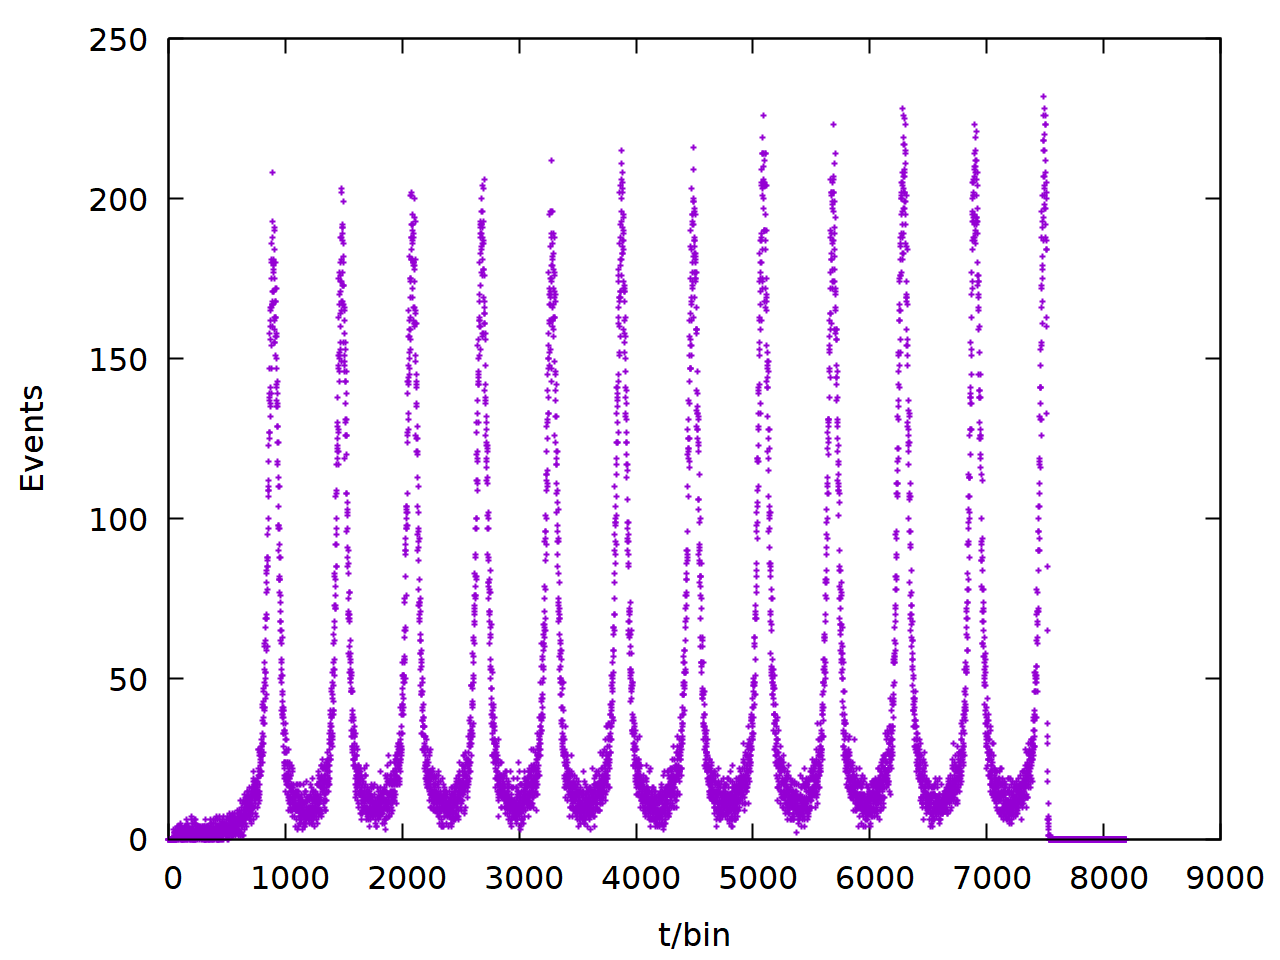
\includegraphics[width=0.7\linewidth]{data/prompt/prompt.png}
\caption{Time calibration measurement -- raw data}
\label{fig:prompt}
\end{figure}

\begin{table}
\centering
\caption{Time calibration measurement -- peak position}
\begin{tabular}{ccc}
\toprule
peak & $t/\si{\nano\second}$ & $t$/bin $\pm 50$/bin\\
\midrule
1&	4&	900\\
2&	8&	1473\\
3&	12&	2104\\
4&	16&	3270\\
5&	20&	3877\\
6&	24&	4472\\
7&	28&	5091\\
8&	32&	5686\\
9&	36&	6281\\
10&	40&	6901\\
\bottomrule
\end{tabular}
\label{tab:prompt}
\end{table}

\begin{figure}
\centering
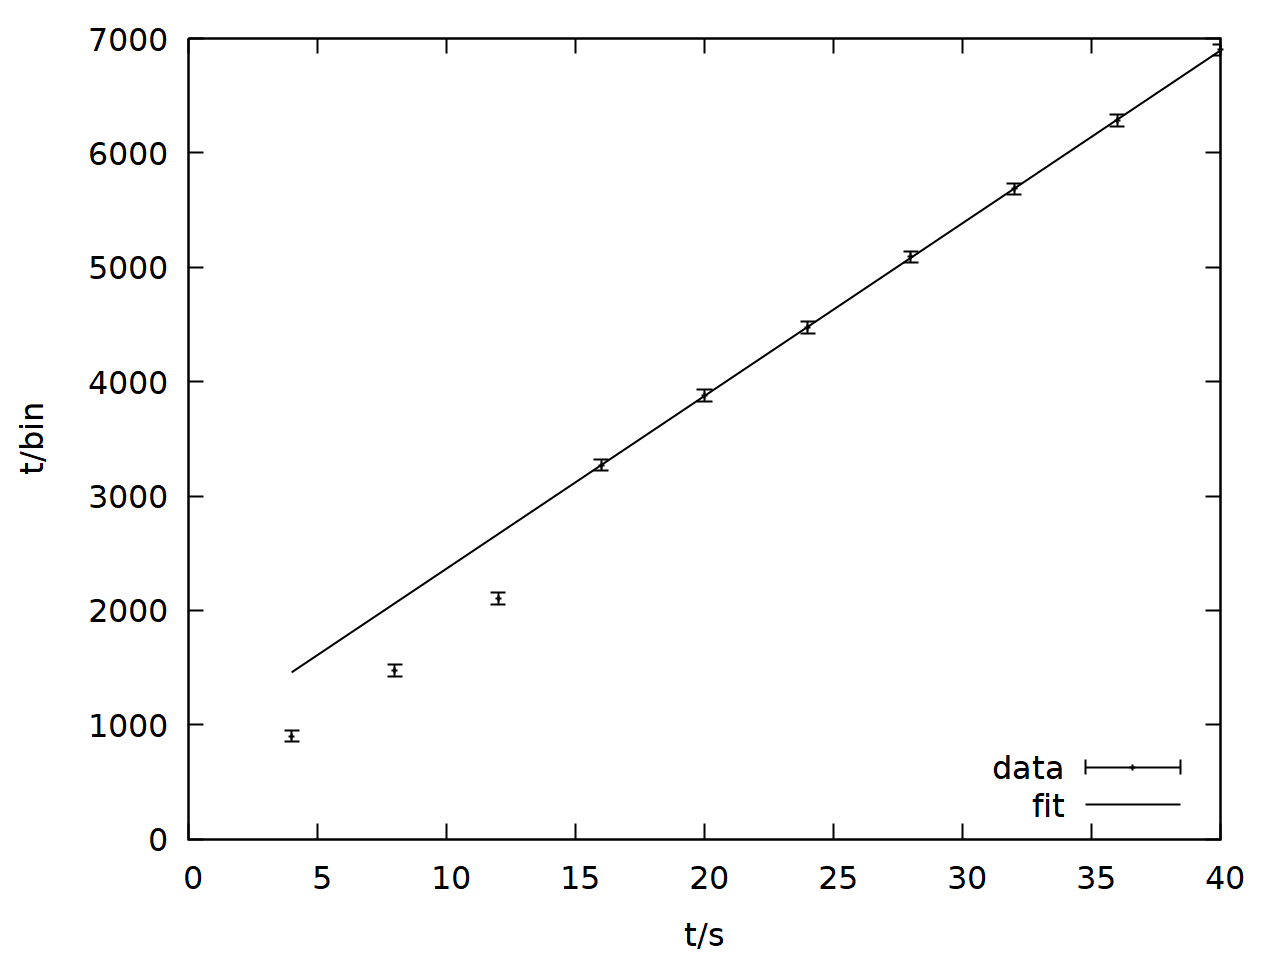
\includegraphics[width=0.7\linewidth]{data/prompt/prompt_fit.png}
\caption{Time calibration measurement -- fit (the three leftmost data points were skipped during the fit)}
\label{fig:prompt_fit}
\end{figure}

In table \ref{tab:prompt} the positions of the peaks are given in bins (We estimated the error to $50$ bins). To find the conversation factor we did a linear fit $a\cdot x + b$ as seen in figure \ref{fig:prompt_fit}. One can see that the points fit perfectly onto that line. However for the first three values there is a small offset. We believe this offset is caused by the nano second delay. We therefore neglected the three leftmost values for fitting. The fit results in $a = (151 \pm 0.3)$ bin/ns and $b = (854 \pm 10)$ bin. This means that $\si{1 \nano\second}$ equals $151$ bins.

\subsection{Time constant of heating system}

To find the time constant of the heating system the heating was set to the lowest level and for 20 minutes every \SI{30}{\second} the temperature was measured ($\Delta T\ind{thermometer} = 0.1 \si{\kelvin}$). The result is given in figure \ref{fig:heatcurve}. Then a exponential fit $B - A \cdot e^{-t/\tau\ind{heat}}$ was executed on that data which resulted in $A = (29.9 \pm 0.2) \si{\kelvin}, B = (55.3\pm 0.1) \si{\celsius}$ and the time constant $\tau\ind{heat} = \si{(245 \pm 4) \second}$. To make sure that the temperature has stabilised within $\Delta T\ind{stabilisation} = 1 \si{\kelvin}$ we decided to wait 10 minutes before starting a measurement at a new temperature (for the indium measurement we changed the temperature by about $10 \si{\kelvin}$). The expected deviation of the temperature is then $\Delta T = 10 \si{\kelvin} e^{-600/245} \approx 0.86 \si{\kelvin} < 1 \si{\kelvin}$. To make sure that the value is inside the error range we choose the error more generously $\Delta T = 1 \si{\kelvin}$.

\begin{figure}
\centering
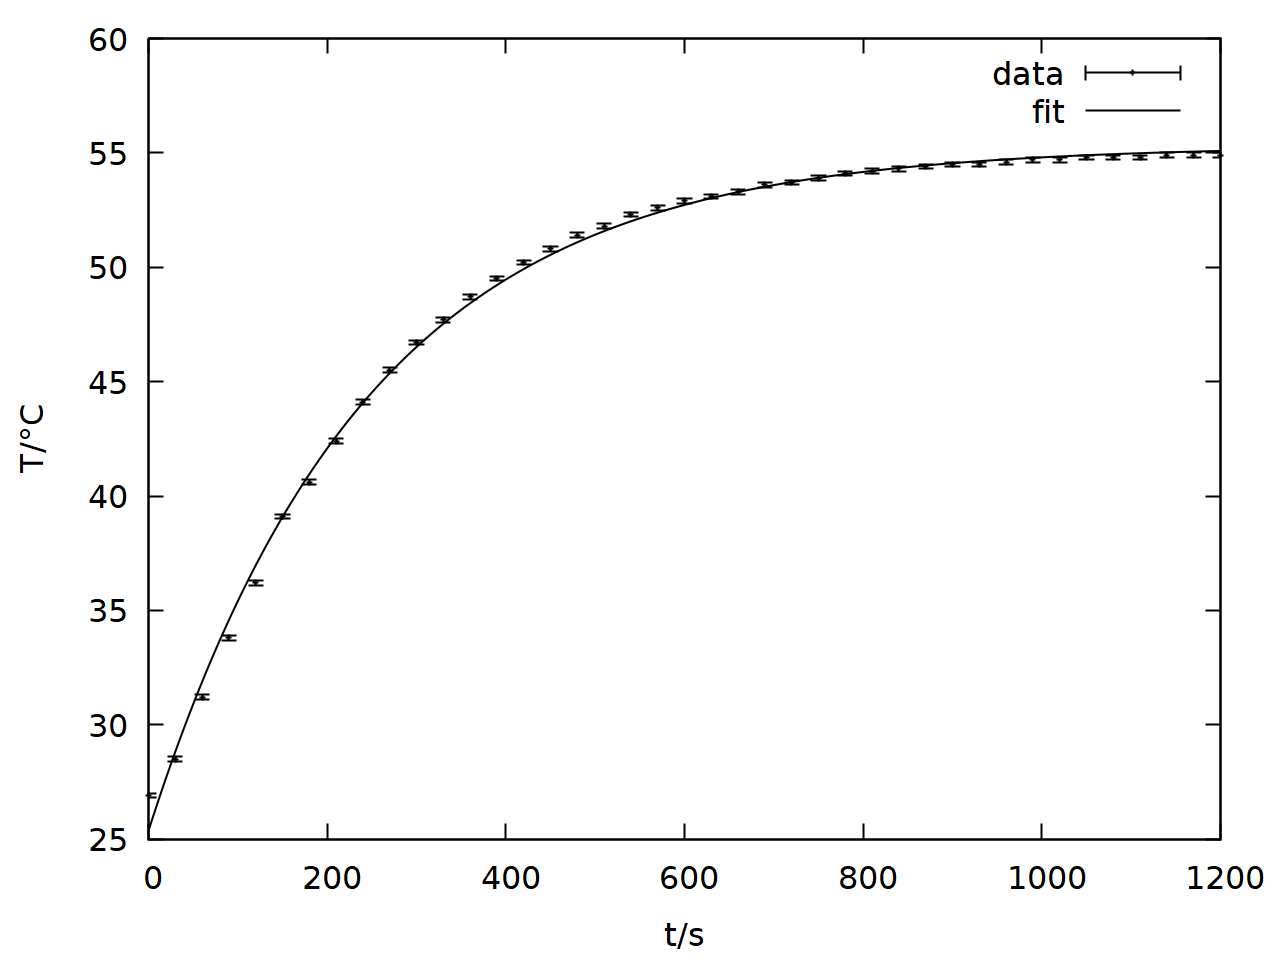
\includegraphics[width=0.7\linewidth]{auswertung/heatcurve.png}
\caption{Measurement to determine the time constant of the heating system}
\label{fig:heatcurve}
\end{figure}

\subsection{Vacancy formation in Indium}

The measured spectra can be found in the appendix. A function according to eq. ?? is fitted to them. The result is given in table \ref{tab:indium_raw}. 

\begin{table}
\centering
\caption{Indium -- fit results}
\begin{tabular}{>{$}c<{$}>{$}c<{$}>{$}c<{$}>{$}c<{$}>{$}c<{$}}
\toprule
T/\si{\celsius} & t_1/\text{bin} & t_2/\text{bin} & A_1/10^3 & A_2\/10^3\\
\midrule
27\pm  1&	99\pm	40&	43\pm	8&	84\pm	57&	144\pm	61\\
55\pm  1&	84\pm	6&	25\pm	4&	74\pm	5&	45\pm	6\\
61\pm	1&	75\pm	4&	20\pm	5&	86\pm	4&	32\pm	5\\
68\pm	1&	86\pm	11&	33\pm	6&	69\pm	14&	49\pm	15\\
78\pm	1&	80\pm	5&	22\pm	5&	81\pm	4&	36\pm	5\\
81\pm	1&	100\pm	20&	43\pm	6&	52\pm	18&	68\pm	19\\
95\pm	1&	88\pm	13&	39\pm	8&	67\pm	20&	50\pm	21\\
108\pm	1&	83\pm 5&	27\pm	5&	81\pm	7&	36\pm	7\\
121\pm	1&	81\pm	5&	23\pm	7&	90\pm	5&	29\pm	6\\
\bottomrule
\end{tabular}
\label{tab:indium_raw}
\end{table}

\begin{figure}
\centering
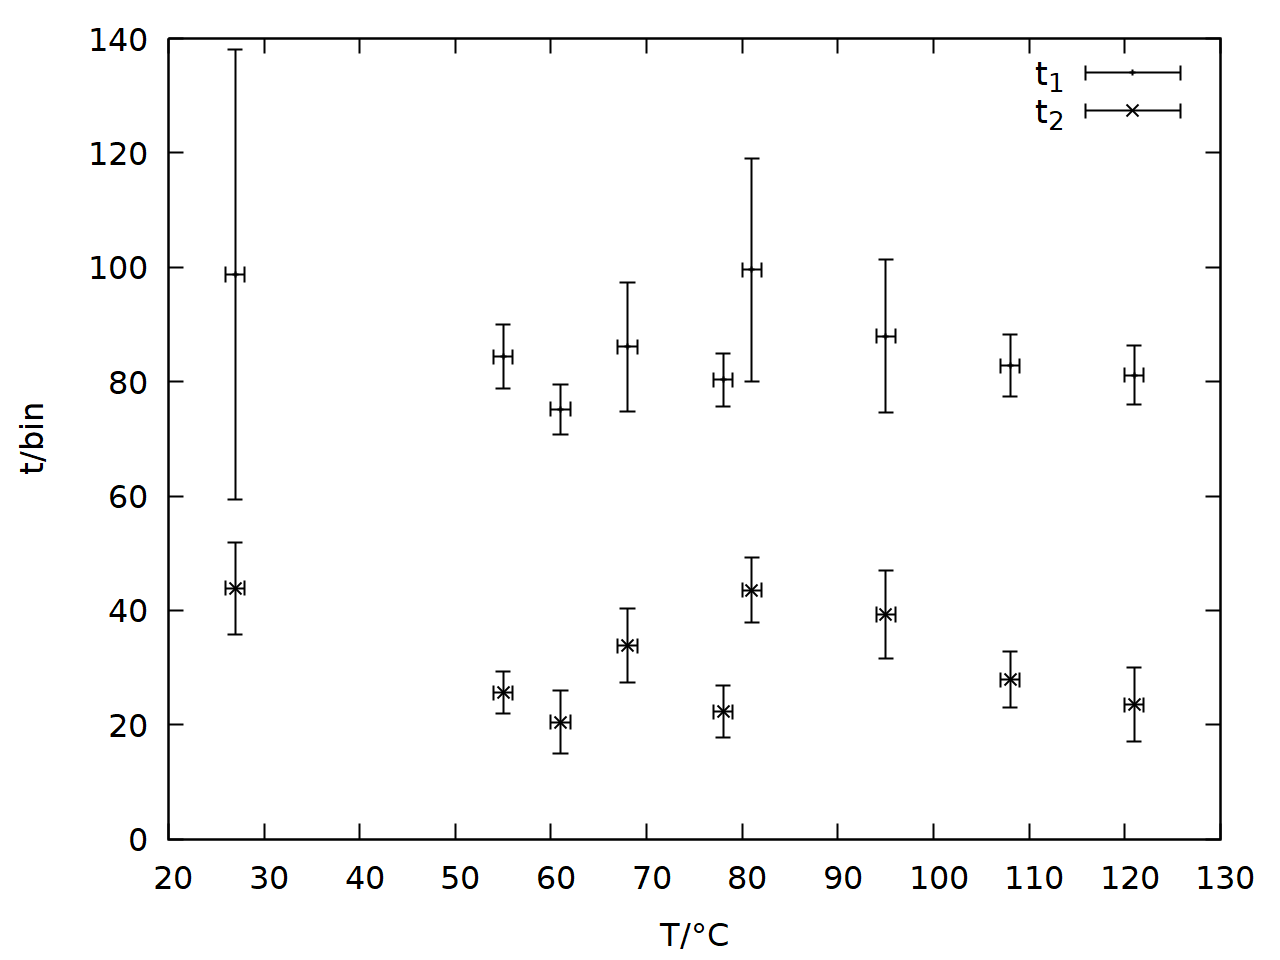
\includegraphics[width=0.7\linewidth]{auswertung/times.png}
\caption{Indium -- $t_1$ and $t_2$ over $T$}
\label{fig:indium_times}
\end{figure}

As one can see in figure \ref{fig:indium_times} the times $t_1$ and $t_2$ are uncorrelated from the temperature. We can not explain this. Since $t_1 > t_2$ we can set $\tau_t = t_1$ and $\tau_0 = t_2$. From these values $\sigma c_t$ can be calculated according to eq. ?? (errors are obtained using gaussian error propagation). Their logarithm is plotted over $1/T[\si{\kelvin}]$ (see figure \ref{fig:indium_res}) and a linear fit $a\cdot x + b$ is obtained. 

\begin{figure}
\centering
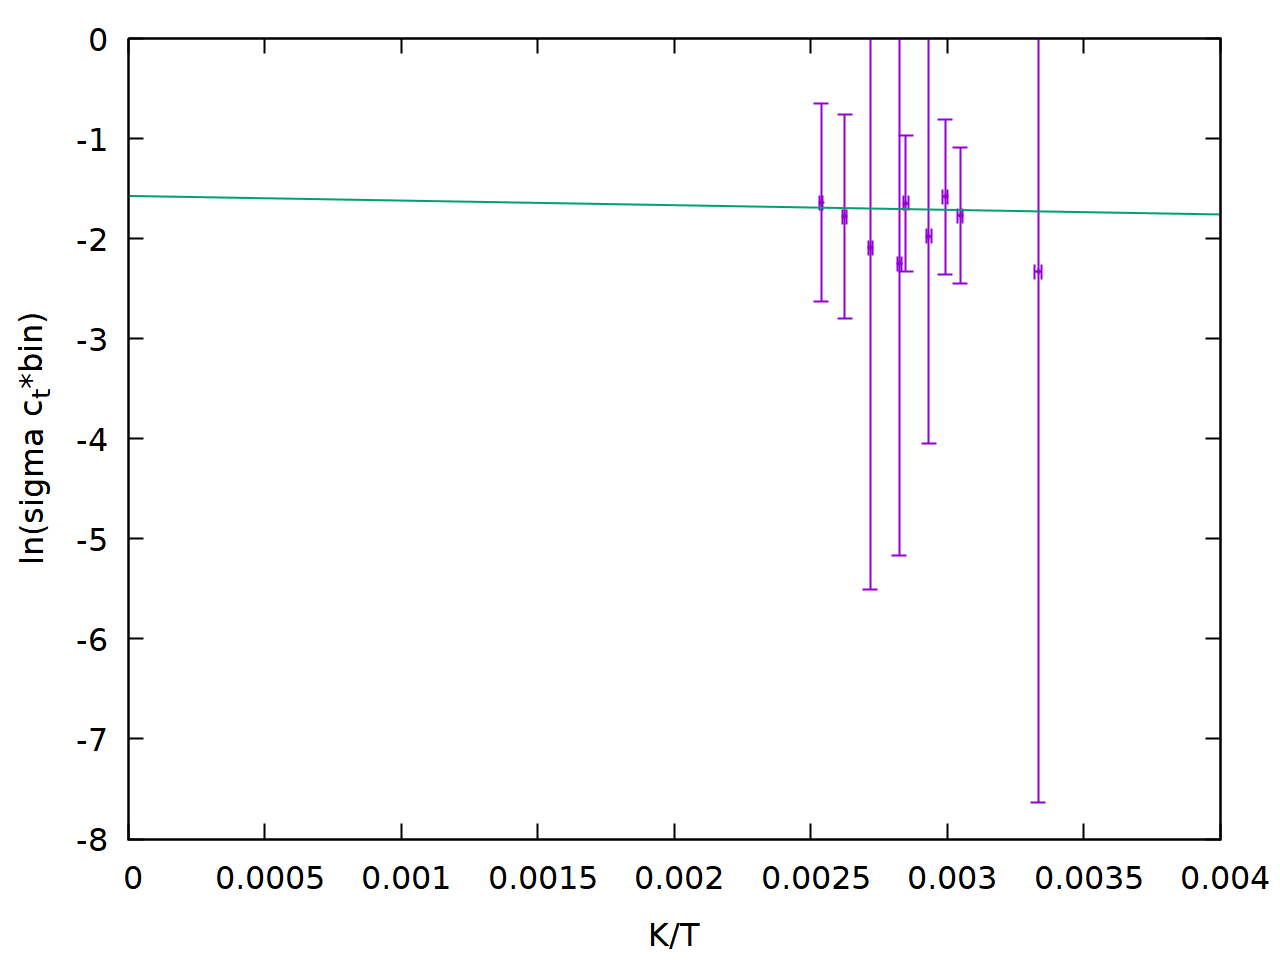
\includegraphics[width=0.7\linewidth]{auswertung/fit.png}
\caption{Indium -- logarithmic plot of $\sigma c_t$ over $1/T$}
\label{fig:indium_res}
\end{figure}

As one can see in figure \ref{fig:indium_res} the data points do not seem to lie on a line. Apart from that the fit results in $a = -H_t/k = (-46 \pm 257) \si{\kelvin}$ and $b = (-1.6 \pm 0.7) + \ln{1/\mathrm{bin}}$. Exponentiating them again yields $\sigma e^{S_t/k} = e^b = (0.21 \pm 0.15) 1/\mathrm{bin} = (32 \pm 23) /\si{\nano\second}$. In \cite{weiler} the value $\sigma e^{S_t/k} = 10^8/\si{\nano\second}$ is given. Our result differs by about 7 orders of magnitude from that. We guess this is because the values of $t_1$ and $t_2$ do not show a sensible dependence of the temperature. Since the fits to the time spectra look suitable we think that the error is caused by the setup of the experiment. However we will ignore this and continue with the evaluation of the experiment.

By multiplying $a$ with $k = 1.38 \cdot 10^{-23}\,\si{\joule/\kelvin}$ \cite{boltzmann} we can find the vacancy formation enthalpy: $H_t = (4 \pm 22) \cdot 10^{-3}\,\si{eV}$. In \cite{enthalpy} the vacancy formation enthalpy is given by $0.56\,\si{eV}$. This means our value differs by two orders of magnitude. But as said before we don't expect our value to be sensible because also the value for $\sigma e^{S_t/k}$ wasn't sensible either. 